\documentclass[sigplan,screen]{acmart}

\usepackage{booktabs}
\usepackage{pgfplots}
\pgfplotsset{compat=1.18}
\settopmatter{printacmref=false}
\renewcommand{\footnotetextcopyrightpermission}[1]{}

\title{Profiling-Guided Optimization of a C++ Ray Tracer}

\author{Yuang Cai}
\author{Yidong Zhang}
\renewcommand{\shortauthors}{Cai and Zhang}

\begin{document}

\begin{abstract}
We optimize a C++ ray tracer using profiling-guided work reduction,
compiler optimization, OpenMP parallelism, and numerical simplification.
The largest improvement comes from replacing per-ray allocation and
sorting with a nearest-hit scan. Subsequent changes improve the numerical
hot path and enable efficient rendering of a 111,748-triangle elephant
scene. All direct correctness comparisons produced byte-identical PPM
output.
\end{abstract}

\keywords{performance engineering, ray tracing, profiling, OpenMP}
\maketitle

\section{Methodology}

We measured the program's \texttt{Total time to create images} timer on a
VM. Piano Room uses one 500$\times$500 frame; Globe uses 24 1000$\times$1000
frames; and Sphere mesh uses one 100$\times$100 frame. The plotted values
are the minimum observed runtime for each version, normalized to the VM
baseline for the same workload. Globe timings exclude movie encoding.
Optimization~1 and~2 were measured once; later reduced-workload results use
the minimum of three runs. The Optimization~5 formal Sphere movie result is
reported separately as a mean of ten runs because it is a different
24-frame workload.

Correctness was checked by comparing PPM output before and after changes.
The direct comparisons reported zero pixel differences and matching SHA-256
hashes. Thus, measured speedups did not come from changing the rendered
image.

\begin{table}[t]
\caption{Absolute runtime and speedup vs. VM baseline.}
\label{tab:runtimes}
\small
\begin{tabular}{@{}lrrr@{}}
\toprule
Version & Piano Room & Globe & Sphere mesh \\
\midrule
Baseline    & 2.3914 s & 150.0140 s & 184.0570 s \\
Opt1        & 1.6311 s (1.47$\times$) & 115.5917 s (1.30$\times$) & 2.9592 s (62.20$\times$) \\
Opt2        & 0.8901 s (2.69$\times$) & 67.9839 s (2.21$\times$) & 1.5679 s (117.39$\times$) \\
Opt3        & 0.2650 s (9.02$\times$) & 35.8627 s (4.18$\times$) & 0.4255 s (432.53$\times$) \\
Opt4        & 0.1963 s (12.22$\times$) & 29.2758 s (5.12$\times$) & 0.3050 s (603.20$\times$) \\
Opt5        & 0.1938 s (12.34$\times$) & 29.3592 s (5.11$\times$) & 0.2853 s (645.19$\times$) \\
\bottomrule
\end{tabular}
\end{table}

\section{Optimizations}

\paragraph{Optimization 1: nearest-hit scan.}
Profiling identified \texttt{calcColor()} as the dominant baseline cost. The
original code allocated a growing intersection array, copied it repeatedly,
sorted all intersections, and consumed only the closest hit. We replaced
this algorithmic/data-structure cost with one linear scan that tracks the
closest finite intersection. This also removes the skybox-path allocation
leak. It is valid for this renderer because shading consumes only the
nearest intersection; it would not apply unchanged to algorithms requiring
all intersections in sorted order. The reduced Sphere mesh runtime fell
from 184.056992~s to 2.959240~s, a 62.20$\times$ improvement.

\paragraph{Optimization 2: optimize core objects with \texttt{-O3}.}
The top-level build used \texttt{-O3}, but core ray-tracer objects from
\texttt{src/Makefile} were compiled at \texttt{-O0}. Rebuilding those
objects with \texttt{-O3} is a compiler optimization that preserves the
algorithm while improving numeric kernels and inlining opportunities. It
reduced Piano Room from 1.631119~s to 0.890050~s and Sphere mesh from
2.959240~s to 1.567893~s. This depends on a conforming optimizing compiler
and does not guarantee identical gains on other architectures.

\paragraph{Optimization 3: OpenMP pixel parallelism.}
Each pixel iteration reads shared scene data and writes a distinct RGB slot,
so we added \texttt{\#pragma omp parallel for} to the image loop and linked
with \texttt{-fopenmp}. This parallelism optimization assumes scene data is
not mutated during rendering and that per-pixel work dominates scheduling
overhead. It improved Sphere mesh from 1.567893~s to 0.425542~s (3.68$\times$)
and Globe from 67.983910~s to 35.862736~s (1.90$\times$). It did not help
the 1$\times$1 Real Elephant benchmark because thread setup dominates such
a tiny workload.

Globe's 1.90$\times$ gain is far below the core count because its perf
profile is not dominated by a single embarrassingly parallel kernel: leading
costs are spread across \texttt{fix(double)} texture-coordinate wrapping,
\texttt{ImageTexture::getColor()} texture sampling, and reflection/lighting
work, each with irregular memory-access patterns from texture lookups. This
mix is more memory-bandwidth- and cache-bound than compute-bound, so adding
threads runs into shared memory-system limits rather than scaling with core
count. Sphere mesh, by contrast, spends nearly all of its time in
self-contained per-ray geometric math with little shared-memory traffic, so
it scales much closer to the core count.

\paragraph{Optimization 4: orthonormal-basis projections.}
\texttt{solveScalers()} was a numerical hotspot after OpenMP. Its callers
provide \texttt{right}, \texttt{up}, and \texttt{vect}, which form an
orthonormal basis; therefore, solving a general 3$\times$3 system is
equivalent to three dot products. We also pass vectors by \texttt{const\&}.
This specialization relies on the basis remaining orthonormal. It reduced
Piano Room to 0.196349~s and Sphere mesh to 0.305031~s. In the post-change
Piano profile, \texttt{solveScalers()} was 10.12\% of self samples, while
lighting and vector operations became the largest costs.

\paragraph{Optimization 5: avoid an unused triangle projection.}
\texttt{Triangle::getIntersection()} used only two components returned by
\texttt{solveScalers()}, so we compute those two dot products directly and
avoid the unused third projection and temporary \texttt{Vector}. This local
work-reduction optimization applies only to triangle intersection; the
light-intersection path still needs its existing calculation. The reduced
Sphere mesh result improved modestly from 0.305031~s to 0.285275~s. The
formal 24-frame Sphere movie averaged 6.975682~s over ten runs. A post-Opt5
100$\times$100 Real Elephant capability run completed in 16.479607~s
(minimum of three runs), but it is not a same-machine baseline comparison.

\begin{figure}[t]
\centering
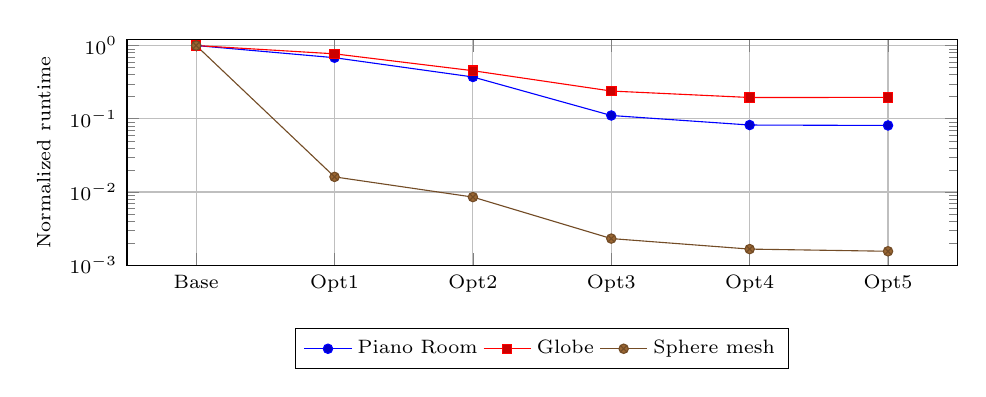
\begin{tikzpicture}
\begin{axis}[
  width=\columnwidth,
  height=1.75in,
  ymode=log,
  log basis y=10,
  ymin=0.001, ymax=1.2,
  ylabel={Normalized runtime},
  symbolic x coords={Base,Opt1,Opt2,Opt3,Opt4,Opt5},
  xtick=data,
  legend style={at={(0.5,-0.28)},anchor=north,legend columns=3,font=\scriptsize},
  grid=major,
  mark size=1.7pt,
  font=\scriptsize
]
\addplot coordinates {(Base,1) (Opt1,0.6821) (Opt2,0.3722) (Opt3,0.1108) (Opt4,0.0821) (Opt5,0.0810)};
\addlegendentry{Piano Room}
\addplot coordinates {(Base,1) (Opt1,0.7705) (Opt2,0.4532) (Opt3,0.2391) (Opt4,0.1952) (Opt5,0.1957)};
\addlegendentry{Globe}
\addplot coordinates {(Base,1) (Opt1,0.01608) (Opt2,0.00852) (Opt3,0.00231) (Opt4,0.00166) (Opt5,0.00155)};
\addlegendentry{Sphere mesh}
\end{axis}
\end{tikzpicture}
\caption{Normalized VM runtime on a logarithmic scale; lower is better.
Sphere mesh uses the reduced one-frame workload.}
\Description{A logarithmic line chart showing decreasing normalized runtime
from baseline through Optimization 5 for Piano Room, Globe, and Sphere mesh.
Sphere mesh drops most sharply after Optimization 1.}
\label{fig:runtimes}
\end{figure}

\section{Results and Introspection}

Figure~\ref{fig:runtimes} shows two distinct phases. First, Optimization~1
eliminated unnecessary work that dominated mesh rendering; a 62.20$\times$
Sphere-mesh speedup is much larger than the 1.47$\times$ Piano improvement
because the mesh repeats the old allocation and sorting work many more
times. Second, Optimization~2--4 improved the remaining per-ray numerical
work and used multiple cores. Optimization~5 is deliberately narrow: it
helps triangle-heavy scenes but has little effect on Piano Room or Globe.

Each optimization was chosen based on what the previous profile showed,
rather than in a fixed order: the baseline profile pointed at allocation and
sorting inside \texttt{calcColor()} (Opt1); once that was removed, the
profile shifted to numeric kernels still compiled without optimization
(Opt2); once those were optimized, the workload was still single-threaded,
so the profile motivated parallelizing the independent per-pixel loop
(Opt3); with parallelism in place, \texttt{solveScalers()} emerged as a
large numerical hotspot (Opt4); and after simplifying it, the profile showed
that \texttt{Triangle::getIntersection()} still computed an unused
projection through the now-cheaper \texttt{solveScalers()} (Opt5). Each step
was thus a prerequisite for the next hotspot to become visible and worth
targeting, rather than a fixed checklist applied up front.

Profiling determined this order. Before Opt1, optimizing a small helper
would have had little impact because \texttt{calcColor()} and allocation
behavior dominated. OpenMP was most effective after each pixel had enough
independent computation to amortize scheduling costs. Potential future work
is acceleration data such as a bounding-volume hierarchy: the large elephant
still linearly scans triangles per ray, but implementing it would be a
larger structural change than the scoped optimizations evaluated here.

\end{document}
